\section{Background research}

Mobile stroke units were first proposed in 2013 by Fassbender et al. \cite{fassbender_mobile_2003}. They were first trialed in Homberg, Germany (published 2015 \cite{walter_diagnosis_2012}), and first test in the US in Houston (published 2015, cite{parker_establishing_2015}.

%%%%%%%%%%%%%%%%%%%%%%%%%%%%%%%%%%%%%%%%%% ECONOMIC BURDEN OF STROKE %%%%%%%%%%%%%%%%%%%%%%%%%%%%%%%%%%%%%%%%%%

\subsection{Economic burden of stroke}

%%%%%%%%%%%%%%%%%%%%%%%%%%%%%%%%%%%%%%%%%% AMBULANCE CALL OUT %%%%%%%%%%%%%%%%%%%%%%%%%%%%%%%%%%%%%%%%%%

\subsection{Ambulance call identification of stroke}

In a 2016 review of dispatch accuracy, Oostema et al \cite{oostema_dispatcher_2016} found "Regardless of the screening tool employed, dispatcher stroke recognition sensitivity was suboptimal (5 studies, range 41-83\%) as was the PPV (7 studies, range 42-68\%)" (see figure \ref{fig:oostema}.

\begin{figure}
    \centering
    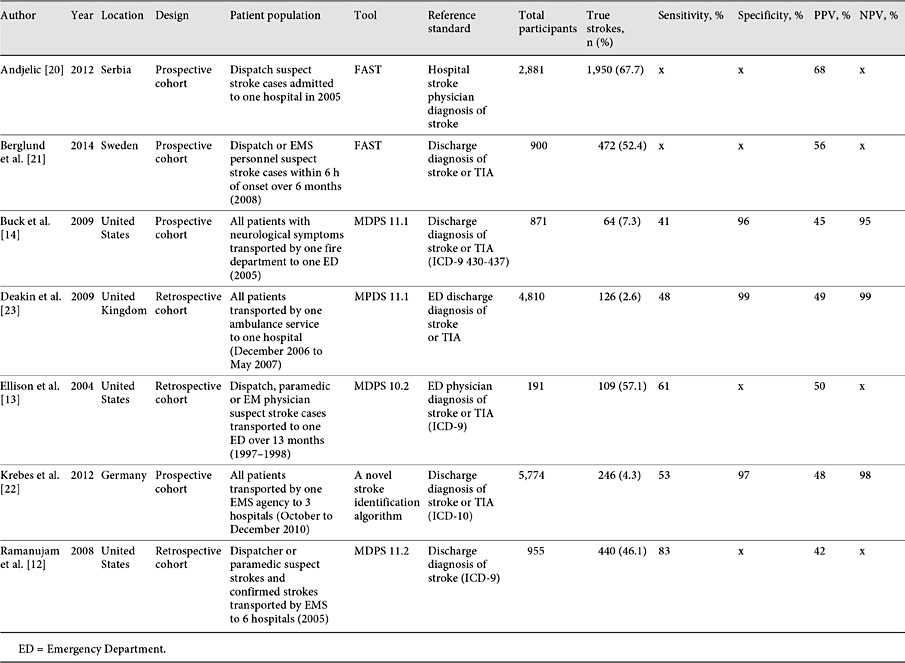
\includegraphics[width=0.9\linewidth]{images_background/oosetema_dispatch_accuracy}
    \caption{Oostema et al figure 2: Ambulance dispatch accuracy}
    \label{fig:oostema}
\end{figure}

In a 2024 review of Emergency Medical Services dispatcher recognition of stroke \cite{wenstrup_emergency_2024}, Wenstrup et al found sensitivity varied from 17.9\% to 83.0\% . Sensitivity median and interquartile range = 56\% (48\%-63\%). PPV was reported in 12 papers and ranged from 24.0\% to 87.7\%. PPV median and interquartile range = 46\% (42\%-50\%).

\begin{figure}
    \centering
    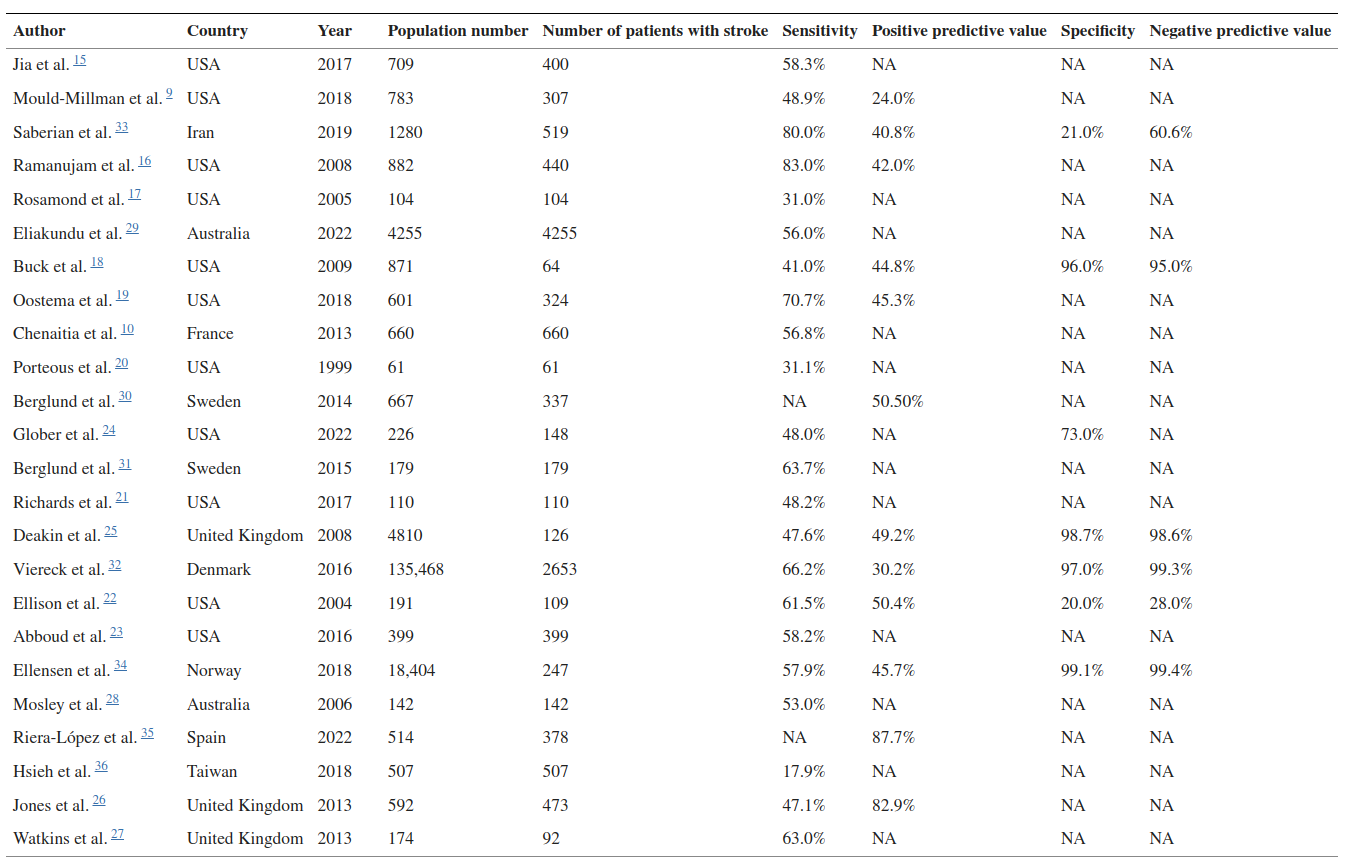
\includegraphics[width=0.75\linewidth]{images_background/wenstrup.png}
    \caption{Wenstrup et al table 1: Ambulance dispatch accuracy}
    \label{fig:wenstrup}
\end{figure}

\subsubsection{UK Studies}

North East Ambulance Service Study \cite{mcclelland_ambulance_2021}: In a study evaluating stroke identification by call handlers and clinicians in the North East Ambulance Service, 2,214 individual cases were analyzed. Call handlers identified acute stroke with a sensitivity of 51.5\% and a positive predictive value (PPV) of 12.8\%, while face-to-face clinicians had a sensitivity of 76.1\% and a PPV of 27.4\% The median on-scene time was 33 (IQR 25–43) minutes.

In a separate study on the North East Ambulance Service \cite{mcclelland_positive_2020} of 5,645 suspect stroke patients identified at call-out, 56\% were confirmed stroke, 6\% were TIA, and 38\% non-TIA stroke mimics.

In a study on the effect of training call handlers \cite{watkins_training_2013}, on 464 patients, sensitivity improved from 63\% to 80\%, but PPV fell from 60.5\% to 39.0\%. 

In a study in North West England \cite{jones_identification_2013} on 592 patients, sensitivity was 45\% and PPV 83\%.

\subsubsection{Stroke recognition systems}

Rudd et al reviewed hospital and pre-hospital stroke recognition system \cite{rudd_systematic_2016}; see figure \ref{fig:rudd}.

\begin{figure}
    \centering
    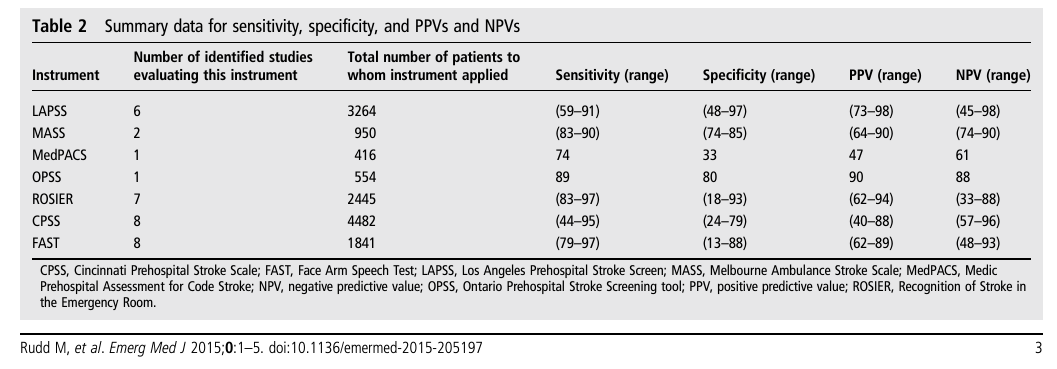
\includegraphics[width=0.9\linewidth]{images_background/rudd.png}
    \caption{Stroke recognition system, from Rudd et al}
    \label{fig:rudd}
\end{figure}

ROSIER (Recognition of Stroke in the Emergency Room):

\begin{itemize}
    \item Facial weakness
    \item Arm weakness
    \item Leg weakness
    \item Speech disturbance
    \item Visual field defects
\end{itemize}



%%%%%%%%%%%%%%%%%%%%%%%%%%%%%%%%%%%%%%%%%% FATIMA METANALYSIS %%%%%%%%%%%%%%%%%%%%%%%%%%%%%%%%%%%%%%%%%%

\subsection{Fatima review and metanalysis on mobile stroke units 2022 \cite{fatima_mobile_2020}
}

A total of 21,297 patients from 11 publications (seven randomized controlled trials and four non-randomized controlled trials including prospective cohort studies) were retrieved. This included 6065 (28.4\%) of the patients treated in the mobile stroke unit and 71.6\% (15,232) of the patients managed in the conventional care.

The mean age at clinical presentation (70.1 vs. 71.05) and National Institute Health Stroke Scale (9.8 vs. 8.4) was comparable (p>0.05) in patients treated with mobile stroke unit and conventional care, respectively.

The mean time-to-treatment window was significantly shorter among the patients treated in mobile stroke unit compared to conventional care (62min vs. 75min; p=0.03, respectively).

The pooled analysis of clinical outcome at day 7 indicated that patients treated in mobile stroke unit had 1.46-folds higher likelihood of better clinical outcome (modified Rankin scale 0–2) than those in the hospital (odds ratio: 1.46, 95\% confidence interval: 1.306–2.03, p=0.02).

However, there was no significant difference in terms of mortality (odds ratio: 0.98, 95\% confidence interval: 0.81–1.18, p=0.80), stroke-related neurological deficits (odds ratio: 1.37, 95\% confidence interval: 0.81–2.32, p=0.24), and other serious adverse events (odds ratio: 0.69, 95\% confidence interval: 0.39–1.20, p=0.19) among patients treated in mobile stroke unit versus conventional care (figure \ref{fig:background_fatima_fig_5}).

\begin{figure}
    \centering
    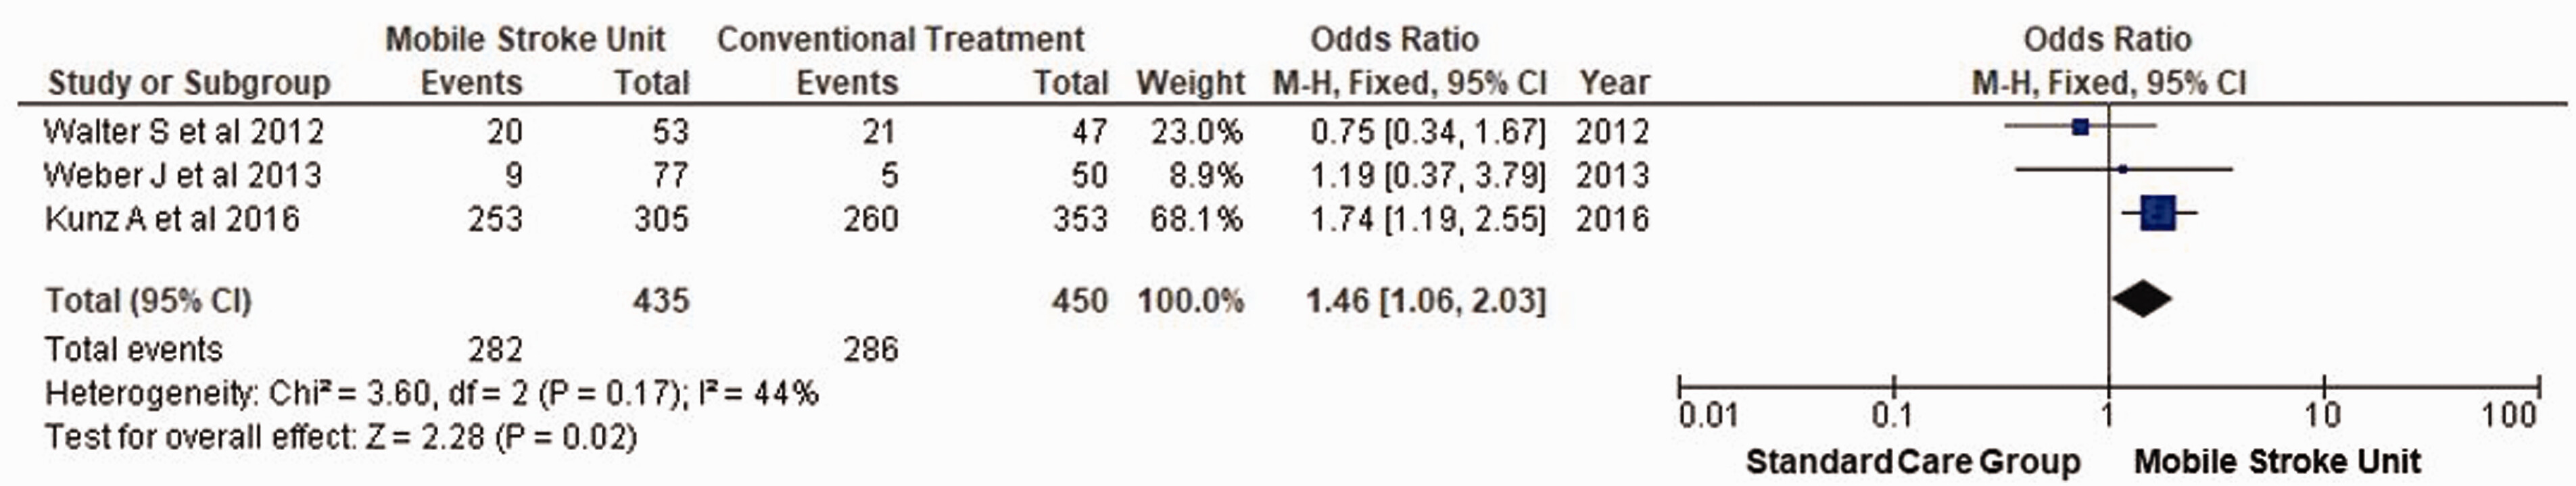
\includegraphics[width=0.5\linewidth]{images_background/fatima_fig_5}
    \caption{Pooled analysis of mRS at 907days (Fatima et al., 2020)}
    \label{fig:background_fatima_fig_5}
\end{figure}

%%%%%%%%%%%%%%%%%%%%%%%%%%%%%%%%%%%%%%%%%% CHEN META-ANLYSIS %%%%%%%%%%%%%%%%%%%%%%%%%%%%%%%%%%%%%%%%%%

\subsection{Chen review and metanalysis on mobile stroke units 2022 \cite{chen_systematic_2022}}

A total of 22,766 patients from 16 publications were included. In total 7,682 (n = 33.8\%) were treated in the MSU and 15,084 (n = 66.2\%) in the conventional EMS.

Economic analysis were available in four studies, of which two were based on trial data and the others on model simulations. The pooled analysis of time metrics indicated a mean reduction of 33 min and 28 minutes in the time-to-therapy and time-to-CT completion, respectively in the MSU.

There was no significant difference on stroke-related neurological events and in-hospital mortality between the MSU and EMS.

The proportion of patients with modified Ranking scale (mRS) of 0–2 at 90 days from onset was higher in the MSU than EMS (p < 0.05, figure \ref{fig:background_chen_fig_5}). The proportion receiving thrombolysis was 27.7\% in EMS and 37.3\% in MSU. Of those receiving thrombolysis, the proportion mRS0-2 was 59.3\% using EMS and 66.2\% using MSU. In all patients, the proportion mRS0-2 was 58.8\% using EMS and 64.5\% using MSU.

\begin{figure}
    \centering
    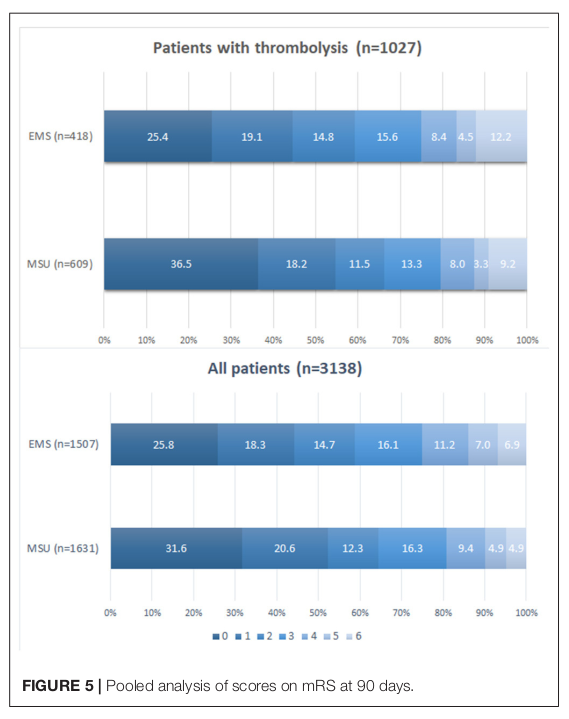
\includegraphics[width=0.5\linewidth]{images_background/chen_fig_5}
    \caption{Pooled analysis of mRS at 90 days (Chen et al., 2021)}
    \label{fig:background_chen_fig_5}
\end{figure}

MSU displayed favorable benefit-cost ratios and incremental cost-effectiveness ratio (\$31,911 /QALY and \$38,731 per DALY) comparing to EMS in multiple economic publications.

%%%%%%%%%%%%%%%%%%%%%%%%%%%%%%%%%%%%%%%%%% INDIVIDUAL TRIALS %%%%%%%%%%%%%%%%%%%%%%%%%%%%%%%%%%%%%%%%%%

\subsection{Individual trials - Germany}

\subsubsection{Walter et al, 2012, Homberg, Germany \cite{walter_diagnosis_2012}}

MSU described in an earlier paper \cite{walter_bringing_2010}.

\begin{figure}[ht]
    \centering
    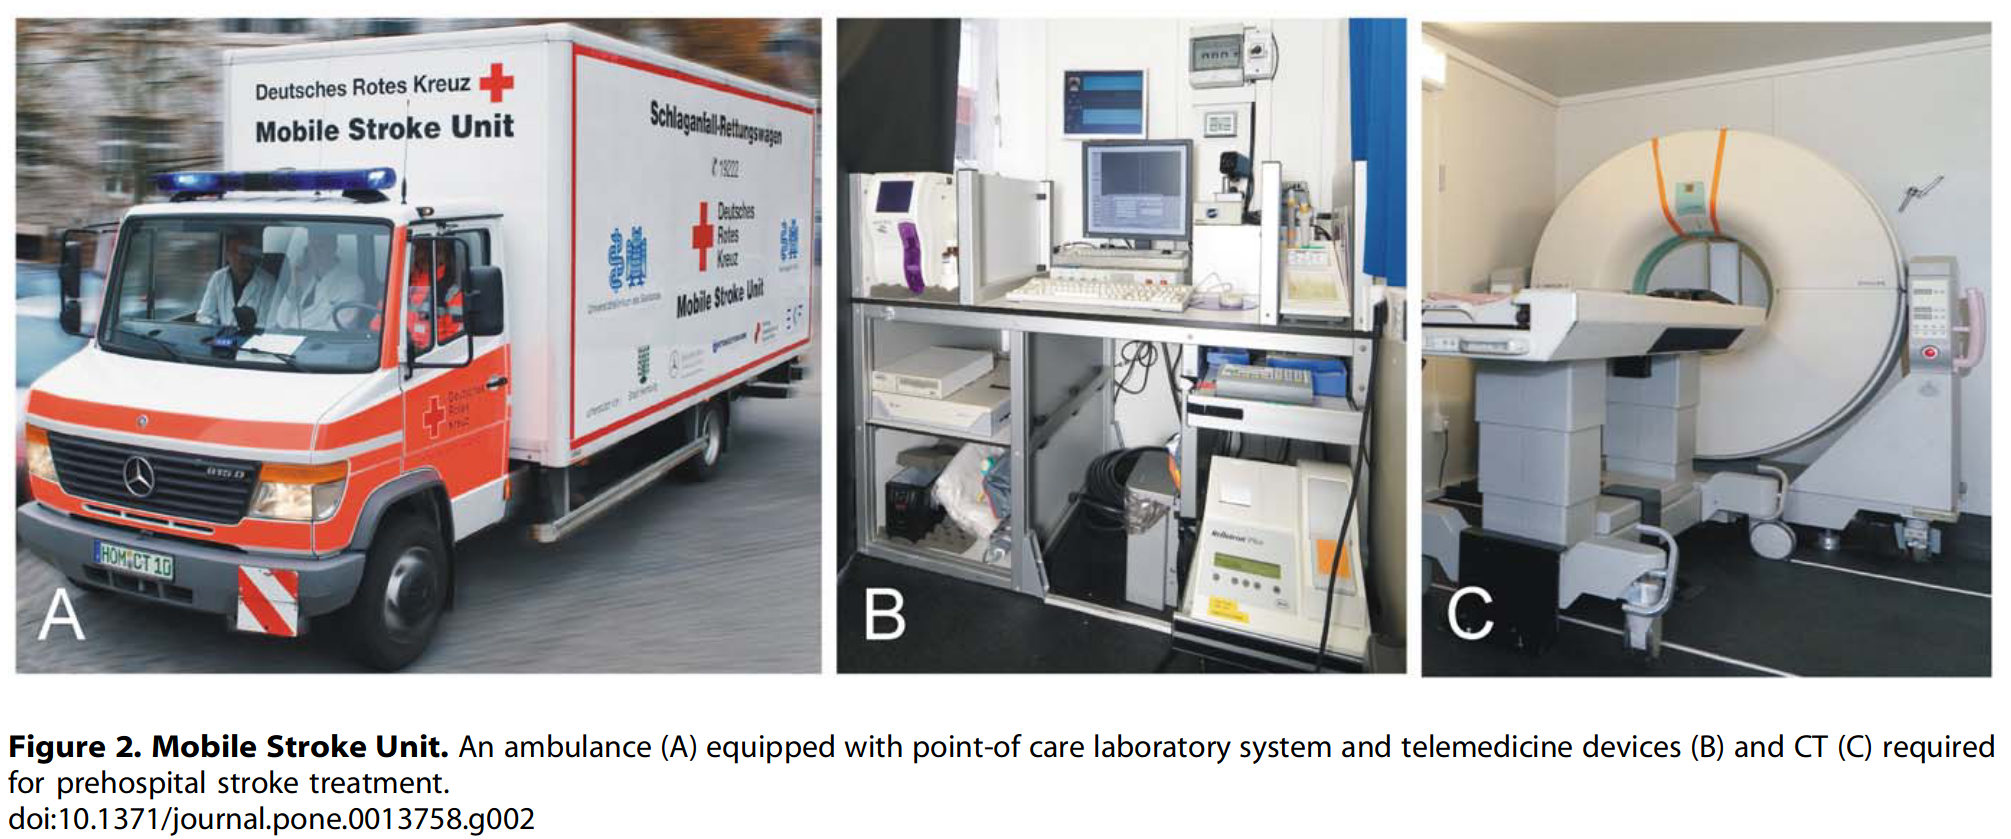
\includegraphics[width=0.95\linewidth]{images_background/walter_msu}
    \caption{The Mobile Stroke Unit, as used by Walter et al.}
    \label{fig:walter_msu}
\end{figure}

Study basics:

\begin{markdown}
* First controlled trial on MSU
* 100 patients (53 MSU, 47 normal care)
* Homberg, Germany (30km radius)
* Dispatch is one symptom of ROSIER: 55\% had confirmed ischaemic stroke, 17\% TIA, 11\% haemorrhage.
* 3 hour onset-to-thrombolysis was used as thrombolysis cut-off
* The MSU team included a paramedic, a stroke physician, and a neuroradiologist
* Primary outcome: therapy decision
\end{markdown}

Results (MSU vs. normal care, with IQR):

\begin{markdown}
* Thrombolysis rate: 23\% vs. 17\% (33\% increased based on un-rounded values)
* Call-to-thrombolysis (min): 38 (34-42) vs. 73 (60-93)
* Symptom onset to therapy decision (min): 56 (43–103) vs. 104 (80–156)
* Call to end of CT (min): 34 (30–38) vs. 71 (62–87)
\end{markdown}

There was no information on call-to-ambulance/MSU arrival times, and MSU or hospital arrival-to-treatment times. But discussion says that at that time arrival-to-thrombolysis target was 60 min, with lots of patients breaching that time. The authors note that MSU strategy provides an opportunity for  blood-pressure management well before hospital arrival.

\subsubsection{Ebinger et al., Berlin, 2014 Timing trial \cite{ebinger_effect_2014}}

\begin{markdown}
* Berlin, Germany
* 6182 adult patients. MSU available in certain weeks
* Thrombolysis rates in ischemic stroke were 29\% (310/1070) during MSU weeks and 33\% (200/614) after MSU deployment vs 21\% (220/1041) during control weeks
* Compared with thrombolysis during control weeks, there was a reduction of 15 minutes in alarm-to-treatment times in the catchment area during STEMO weeks (76.3 min vs 61.4 min P < .001).
* Among patients for whom STEMO was deployed, mean alarm-to-treatment time (51.8 min) was shorter by 25 minutes than during control weeks.
* MSU deployment incurred no increased risk for intracerebral hemorrhage 
\end{markdown}

\subsubsection{Wendt et al., Berlin \cite{wendt_improved_2015}}

Focus is on delivering patients to the right hospital:

\begin{markdown}
* Berlin
* Normal care and MSU care week
* 1804 of 6182 (29\%) patients received MSU care and 4378 of 6182 (71\%) patients conventional care.
* 245 of 2110 (11.6\%) patients with cerebrovascular events were sent to hospitals without Stroke Unit in conventional care when compared with 48 of 866 (5.5\%; P<0.01) patients in MSU care.
* The delivery rate of patients with intracranial hemorrhage to hospitals without neurosurgery department was 43.0\% (65 of 151) in conventional care and 11.3\% (7 of 62) in MSU care (P<0.01).
* 89\% sensitivity, and 77\% specificity for pre-hospital diagnosis of stroke/TIA (79\% PPV, 87\% NPV)
\end{markdown}

\subsubsection{Ebinger et al., Berlin, 2015 \cite{ebinger_effects_2015}}

* The MSU was staffed with a neurologist trained in emergency medicine, a
paramedic, and a radiology technician. A neuroradiologist was on call to evaluate images acquired on board the STEMO via a teleradiology connection.
* Thrombolysis rates in ischemic stroke were 200 of 614 patients (32.6\%) when MSU was deployed and 330 of 1497 patients (22.0\%) when conventional care was administered (P < .001).
* Among all patients who received thrombolysis, the proportion of golden hour thrombolysis was 6-fold higher after MSU deployment (62 of 200 patients [31.0\%] vs 16 of 330 [4.9\%]; P < .01).
* Compared with patients with a longer time from symptom onset to treatment, patients who received golden hour thrombolysis had no higher risks for 7- or 90-day mortality (adjusted odds ratios, 0.38 [95\% CI, 0.09-1.70]; P = .21 and 0.69 [95\% CI, 0.32-1.53]; P = .36) and were more likely to be discharged home (adjusted odds ratio, 1.93 [95\% CI, 1.09-3.41]; P = .02).
* No detailed comparison or breakdown of times was given.

\subsubsection{Travel times in Berlin \cite{koch_influence_2016}}

With increasing distance from MSU base:

* Time from call to hospital arrival increases in comparison with normal care
* Catchment population increases in proportion to square of radius
* Call to treatment increases, but was better than normal care in all zones, but advantage dropped from 35 mins (zone 1) to 18 minutes (zone 4)

* MSU 8-18 minutes call-to-arrival, 25 mins from arrival to completion of imaging (35-50 min call to imaging), and 35-40 mins arrival to treatment (40-60 min call-to-treatment).
* Normal care about 7 min call to ambo arrival, 35 min call to hospital arrival, 40-45 min door-t-needle, 75-80 min call-treatment


\begin{figure}
    \centering
    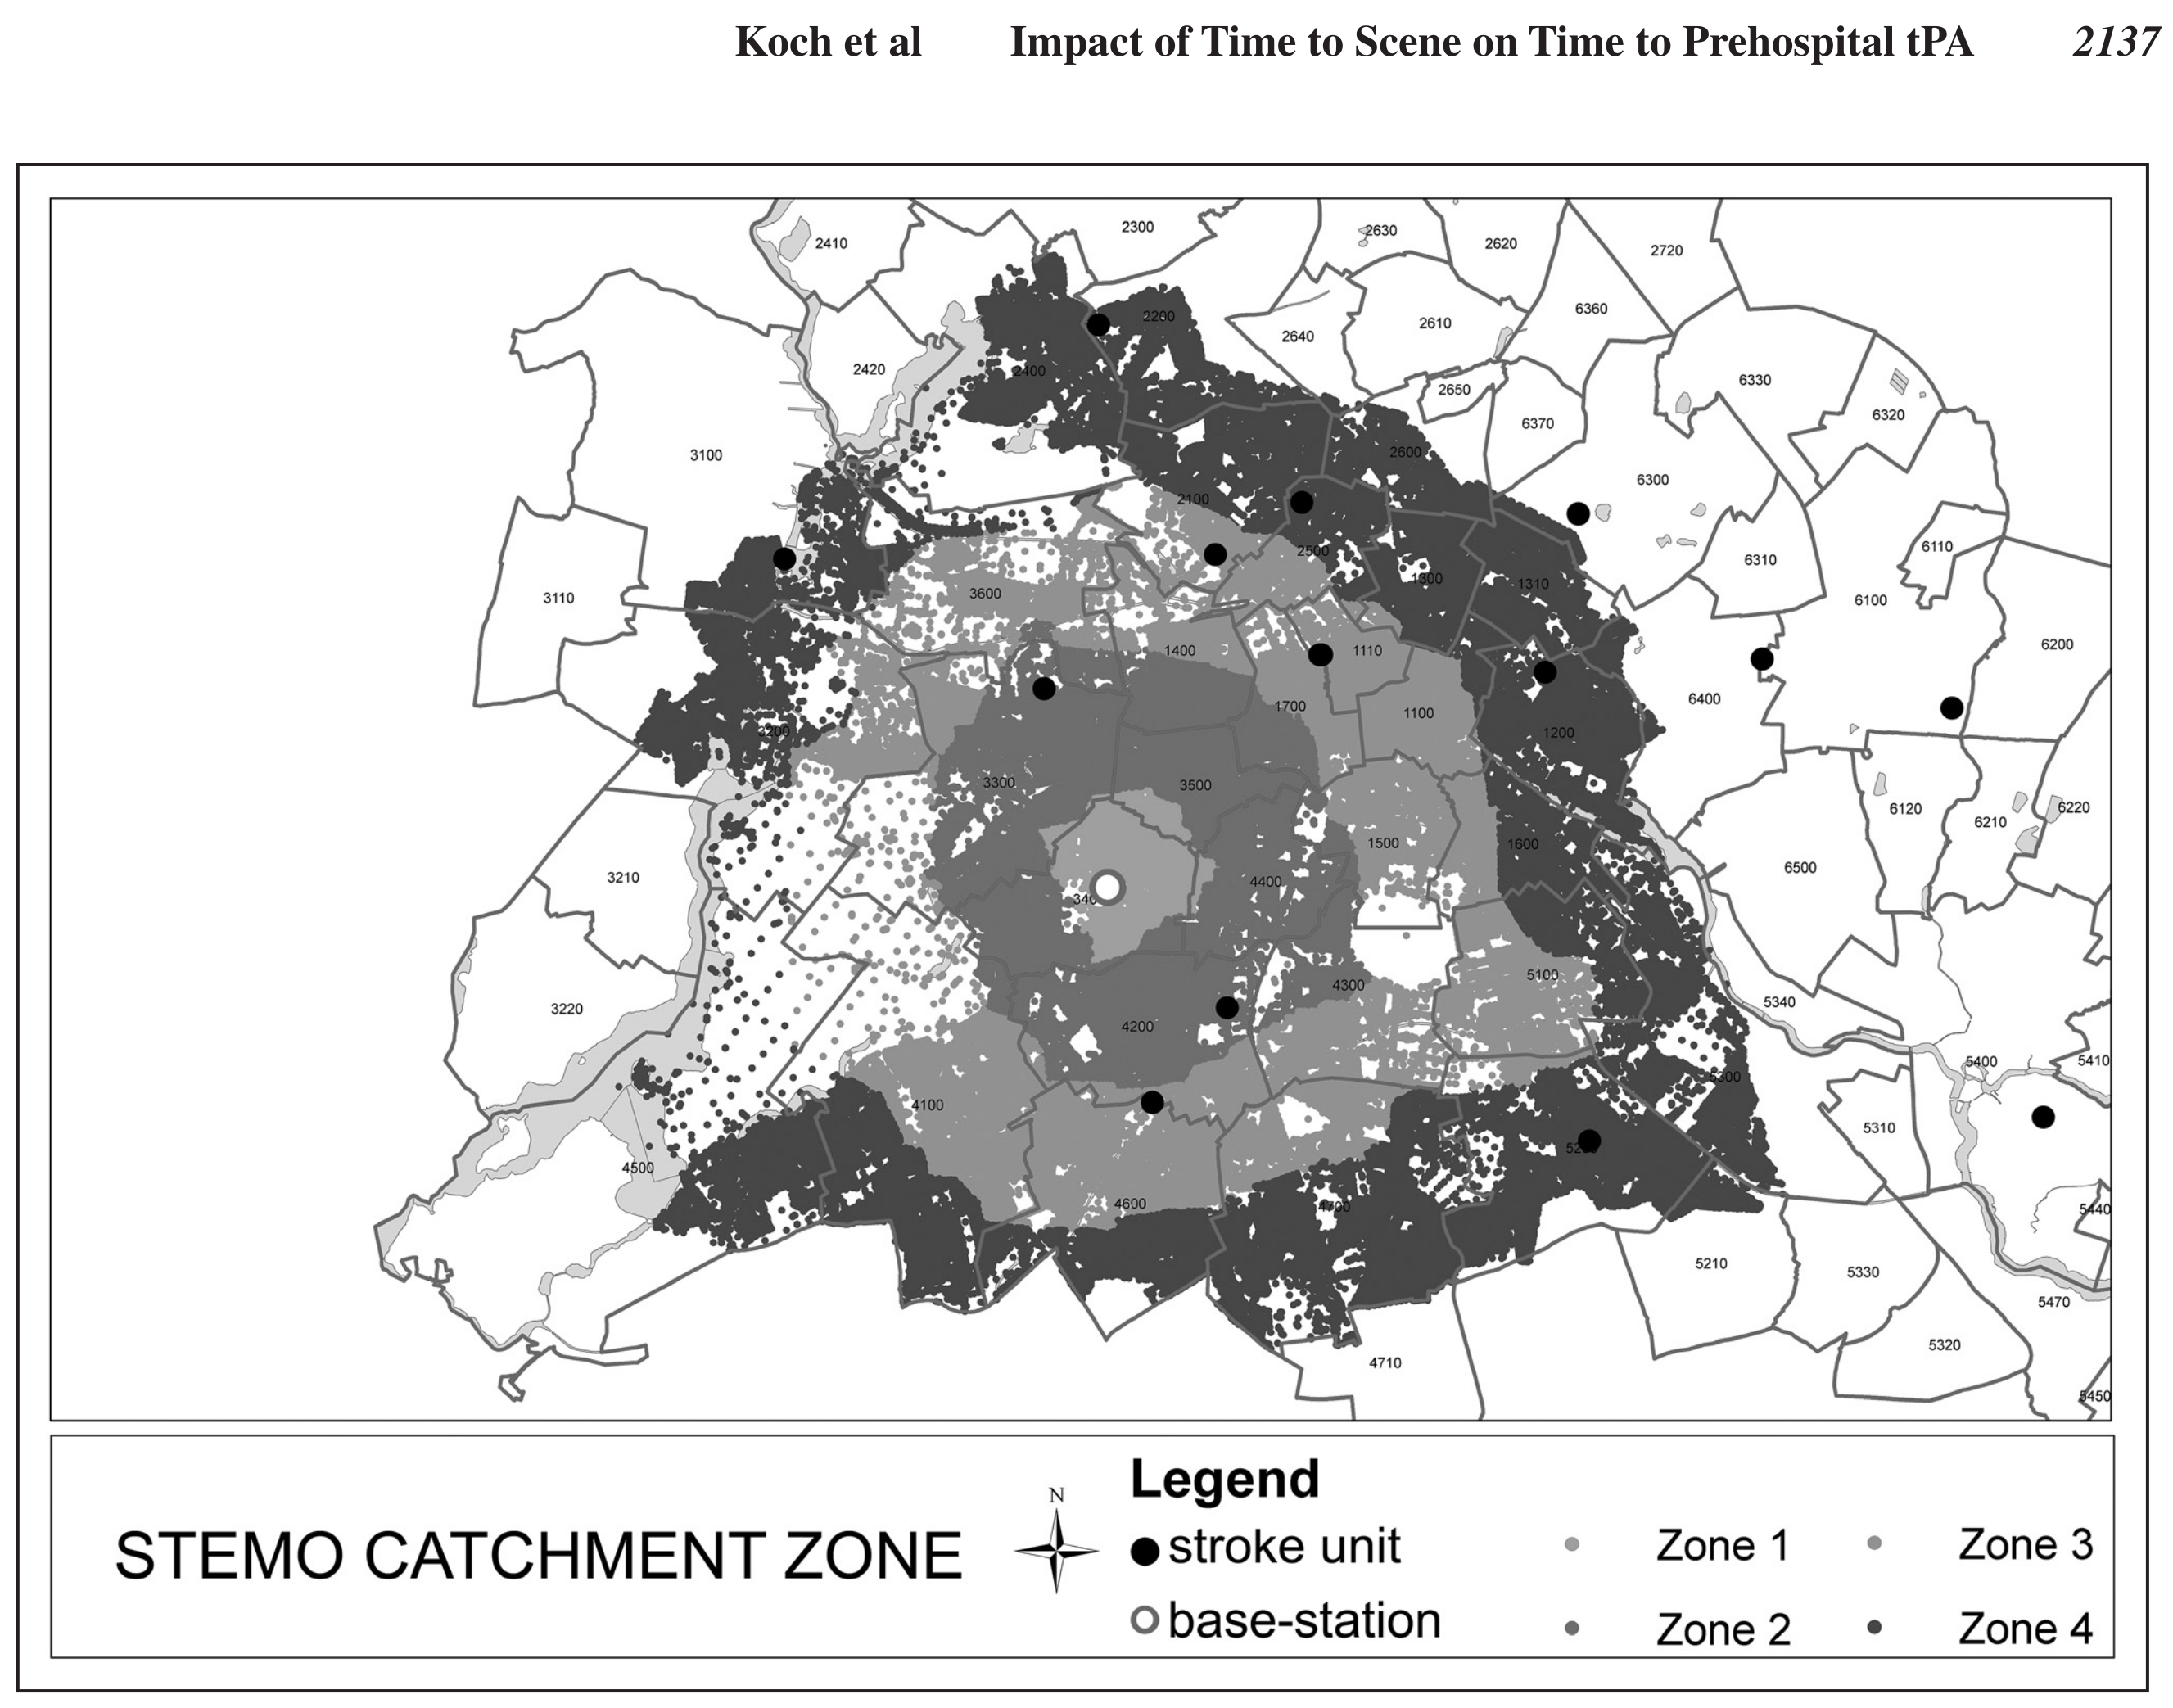
\includegraphics[width=0.9\linewidth]{images_background/berlin_map_2.png}
    \caption{Map of Berlin MSU study area }
    \label{fig:map_berlin_2}
\end{figure}

\begin{figure}
    \centering
    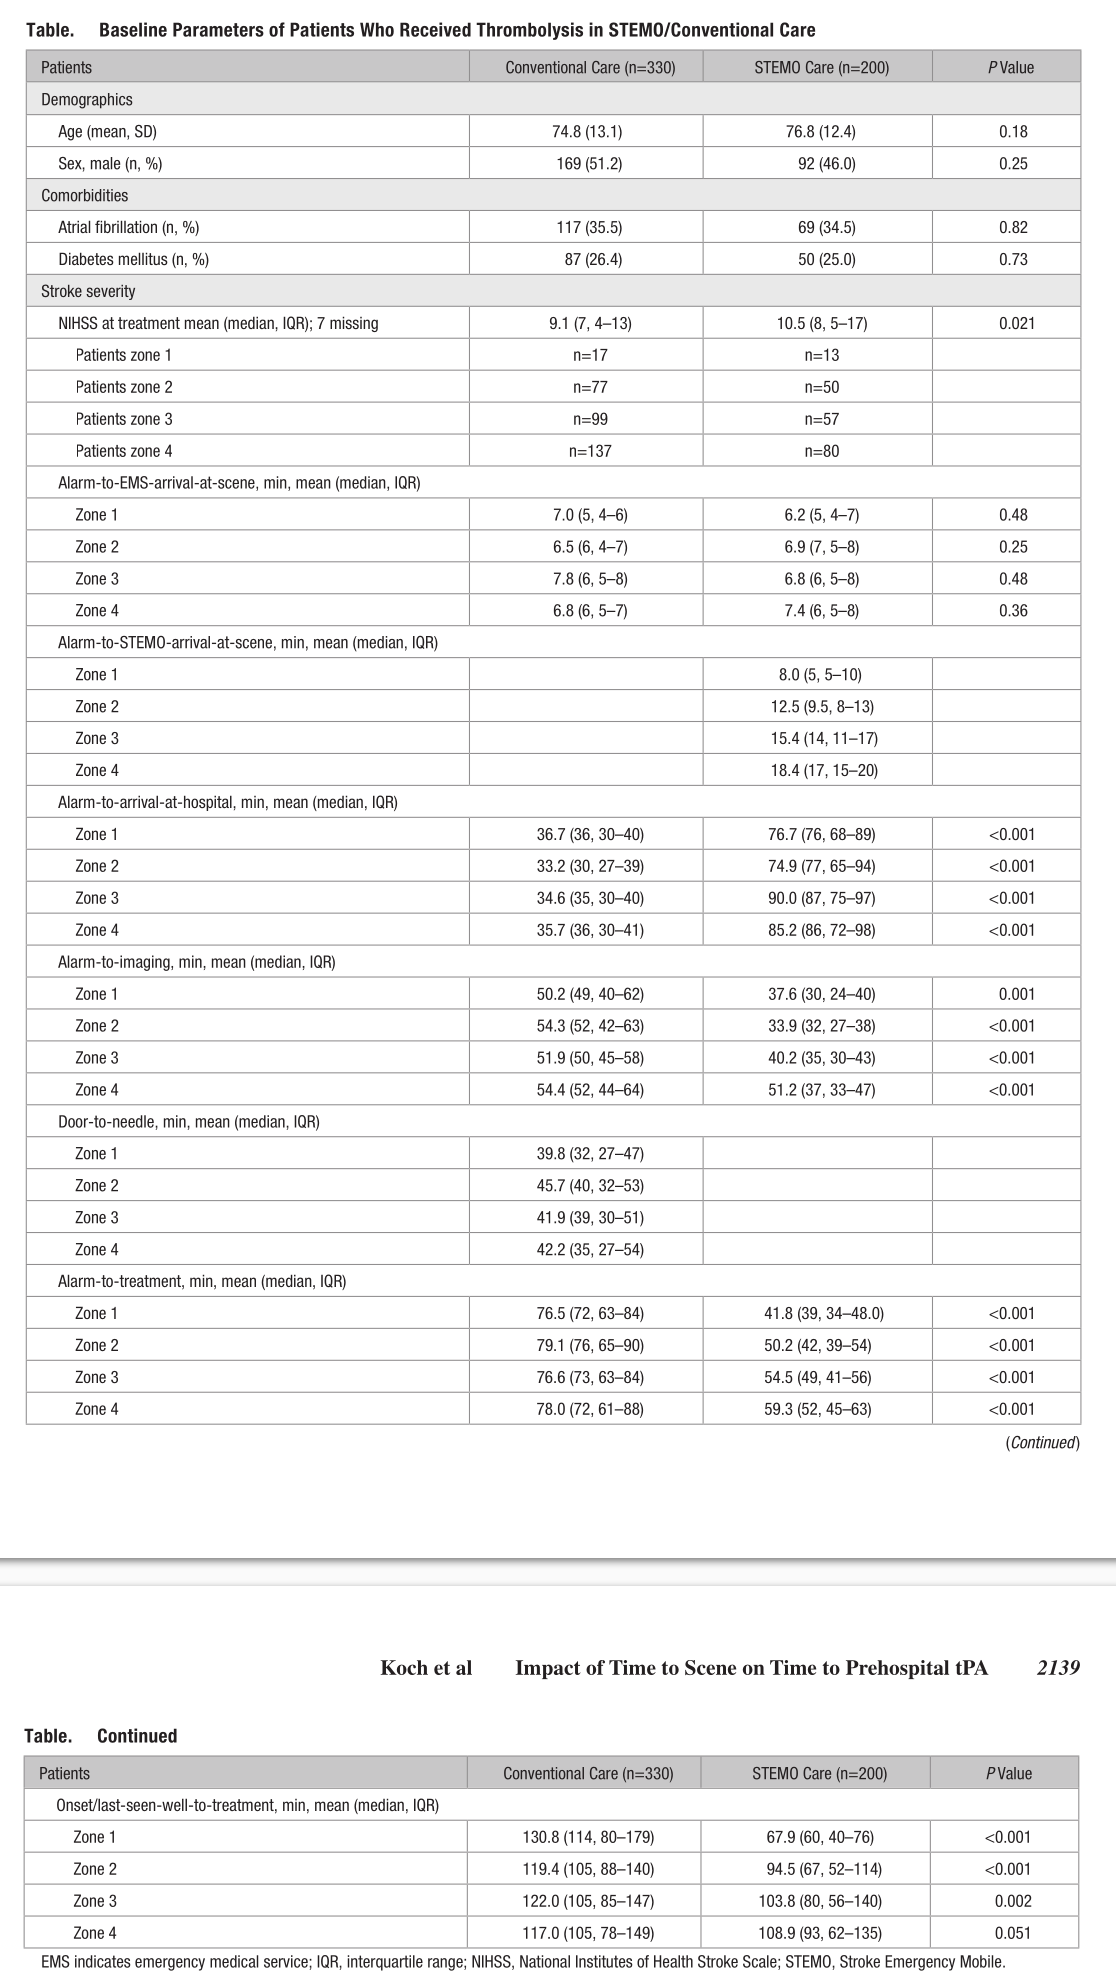
\includegraphics[width=0.5\linewidth]{images_background/koch_timings.png}
    \caption{Timing from Berlin study; from Koch et al.}
    \label{fig:kock_timings}
\end{figure}

\subsubsection{Kunz et al., Berlin, Observational study \cite{kunz_functional_2016}}

* Logistic regression analysis
* The primary outcome was the proportion of patients who had lived at home without assistance before stroke and had a 3-month modified Rankin Scale mRS) score of 1 or lower.
* Findings:  Between Feb 5, 2011, and March 5, 2015, 427 patients were treated within the MSU vehicle and their data were entered into a pre-hospital registry. 505 patients received conventional care and their data were entered into an in-hospital thrombolysis registry. Of these, 305 patients in the MSU group and 353 in the conventional care group met inclusion criteria and were included in the analysis. 161 (53\%) patients in the MSU group versus 166 (47\%) in the conventional care group had an mRS score of 1 or lower (p=0·14). Compared with conventional care, adjusted odds ratios (ORs) for MSU care for the primary outcome (OR 1·40, 95\% CI 1·00–1·97; p=0·052) were not significant. Intracranial haemorrhage (p=0·27) and 7-day mortality (p=0·23) did not differ significantly between treatment groups.
* Interpretation We found no significant difference between the proportion of patients with a mRS score of 1 or lower receiving MSU care compared with conventional care. However, our results suggest that pre-hospital start of intravenous thrombolysis might lead to improved functional outcome in patients. This evidence requires substantiation in future large-scale trials.

Comparison was MSU or normal ambulances and in-hospital care at the Charité Campus Benjamin Franklin in Berlin (see fig \ref{map_berlin_1}).

\begin{figure}
    \centering
    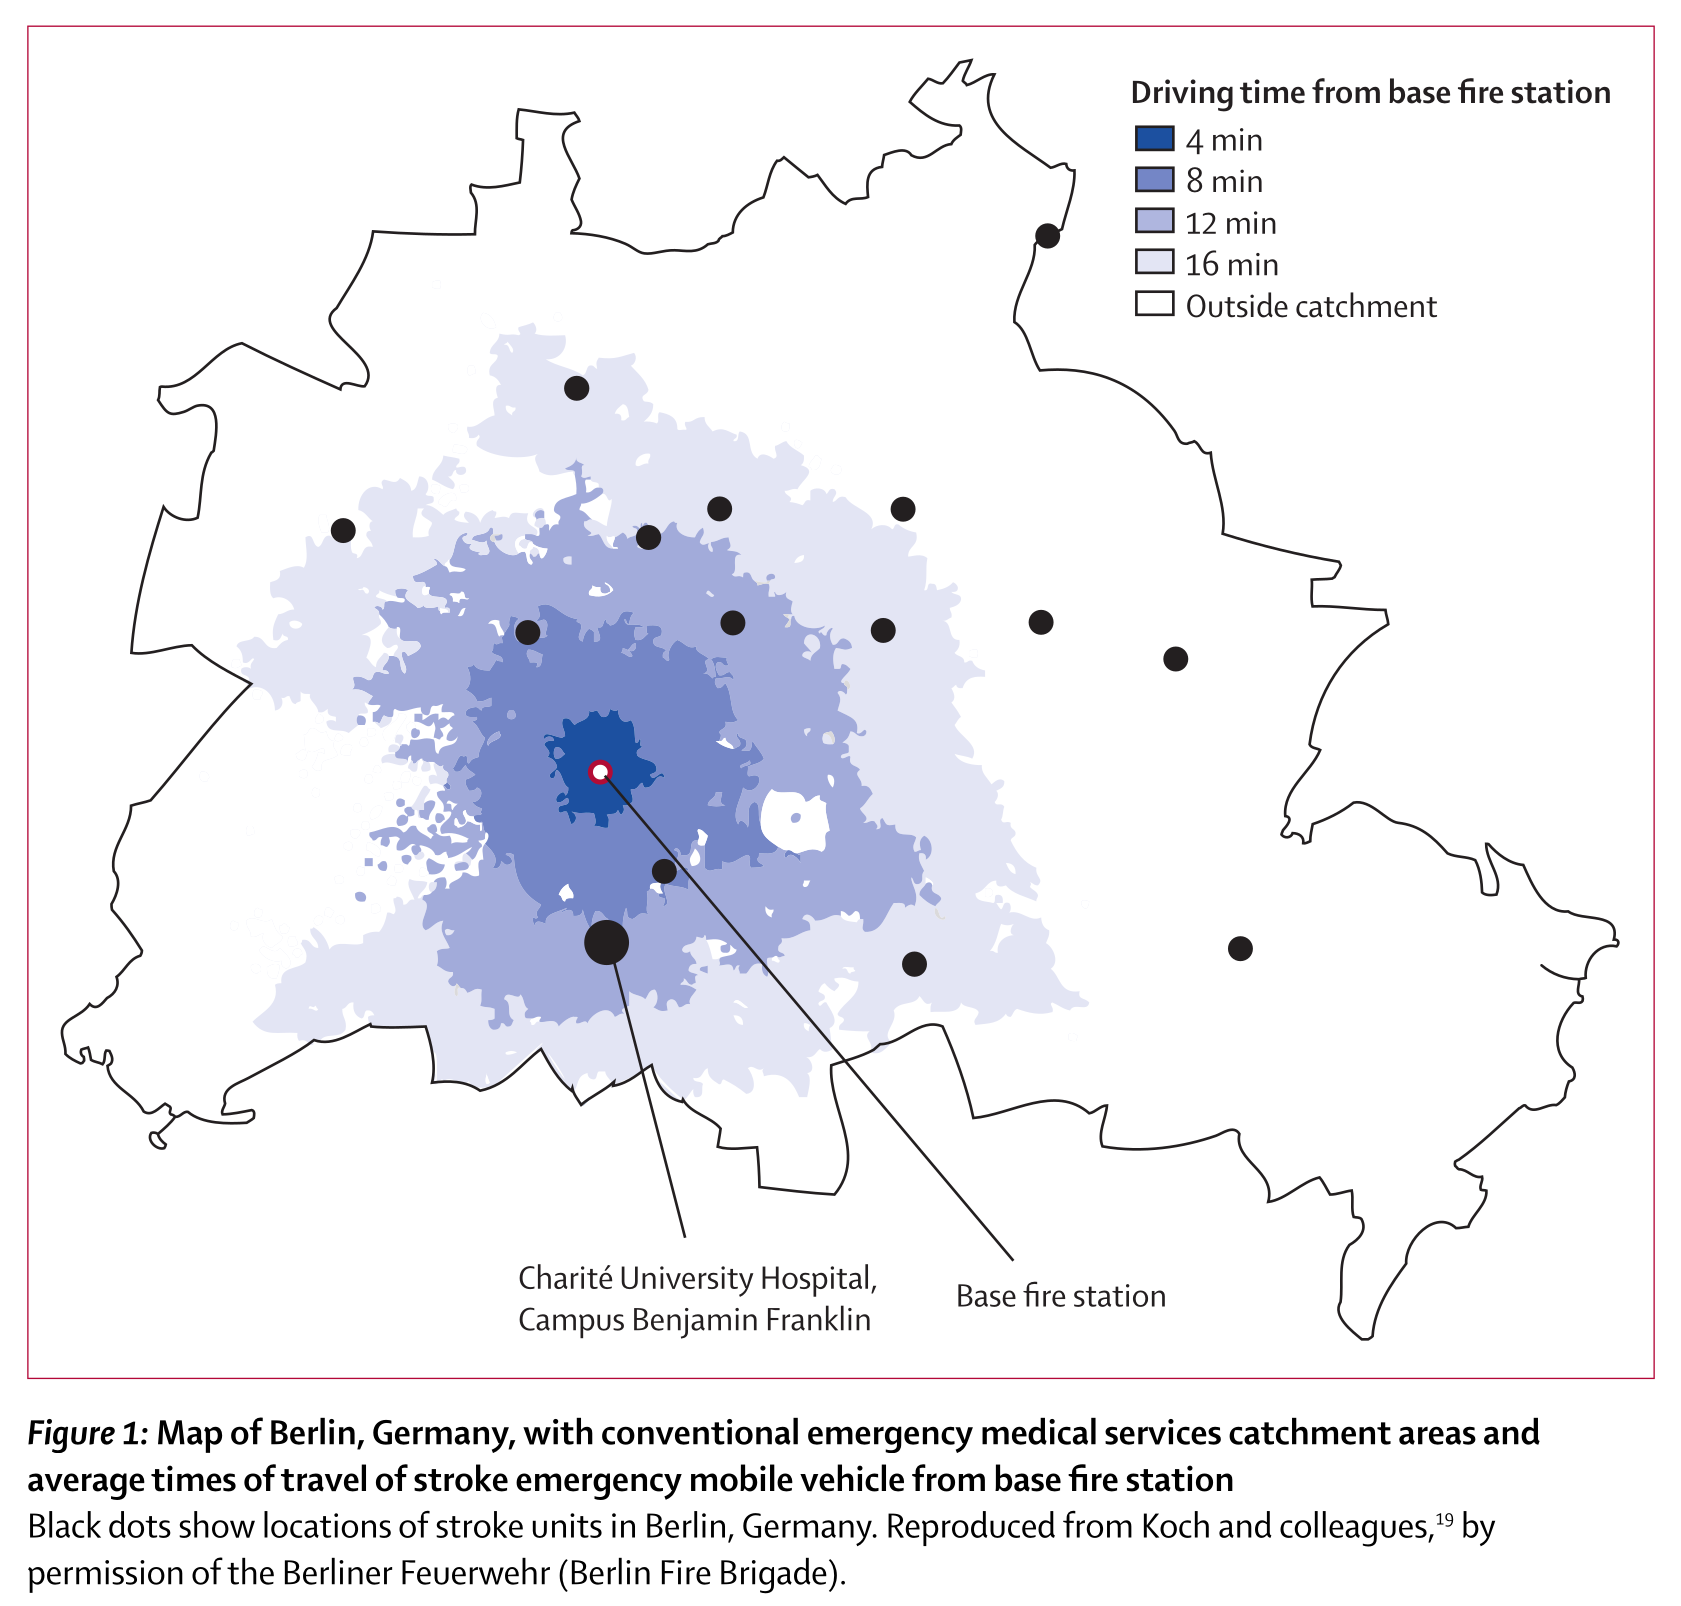
\includegraphics[width=0.5\linewidth]{images_background/berlin_map_1_.png}
    \caption{Map of Kunz et al. observational study area. MSU vs. care at the Charité Campus Benjamin Franklin in Berlin }
    \label{fig:map_berlin_1}
\end{figure}


\subsubsection{Ebinger et al., Berlin, 2021 Outcome trial \cite{ebinger_association_2021}}

\begin{markdown}
* Berlin, Germany
* Non-blind: Use a MSU if available (but not available for 44\% of calls)
* 1,543 patients (749 MSU, 794 normal care)
* Primary outcome: Distribution of mRS scores
\end{markdown}

Results (MSU vs. normal care, with IQR):

\begin{markdown}
* Lower median mRS at 3 months (mRS 1 vs 2)
* MSU had lower 3-month  disability scores: 80.3\% had none to moderate disability; 12.6\% had severe disability; and 7.1\% had died vs patients without an MSU dispatched: 78.0\% had none to moderate disability; 13..3\% had severe disability; and 8.8\% had died (common OR for worse functional outcome, 0.73, 95\% CI, 0.54-0.99; P = .04).
* Dispatch to MSU/ambo arrival (mins) 15 (12-19) vs 8 (6-10)
* Dispatch to hospital arrival (mins) 67 (46 to 82) vs 37 (31 to 44)
* Thrombolysis use: 60.2\% vs 48.1\%
* Thrombolysis dispatch to IVT mins: 50 (43 to 64) vs. 70 (59 to 86)
* Imaging to IVT: 12 (7 to 22) vs 15 (10 to 23)
* Door-to-needle (normal care) mins: 30 (22-40)
* Thrombectomy use: 13.8\% vs 14.2\%
* Dispatch to thrombectomy mins: 137 (117 to 166) vs 125 (110 to 154)
\end{markdown}


\subsection{Individual trials - USA}

\subsubsection{Parker at al., Houston, US, 2015 \cite{parker_establishing_2015}}

\begin{markdown}
* Houston, Texas
* Pilot study to establish MSU
* Describes challenges in establishing MSU
\end{markdown}

\subsubsection{Borey et al., Houston, 2018 \cite{bowry_time_2018}}

Bowry et al \cite{bowry_time_2018} compared time from MSU arrival to decision in 50 patients in Houston. Time to tPA decision for the TM-VN was 21 minutes (interquartile range, 16.25–26) versus 18 minutes (interquartile range, 14–22) for the OB-VN (P=0.01). Initiation of tPA bolus was 24 minutes (interquartile range, 19.75–30) for the TM-VN versus 24 minutes (interquartile range, 19–27.75) for the OB-VN (P=0.5).

\subsubsection{BEST-MSU study, 7 US citiesd 2021 \cite{grotta_prospective_2021}}

Seven US cities:

1. Houston, Texas
2. Memphis, Tennessee  
3. Denver, Colorado
4. Los Angeles, California
5. New York, New York
6. Indianapolis, Indiana
7. Burlingame, California (San Mateo County)

Patients were considered to be enrolled if they met screening criteria for t-PA treatment on MSU or EMS arrival at the scene, whether or not they became eligible for the primary outcome analysis. Each MSU was staffed by one or two paramedics, a CT technologist, and a critical care nurse. A vascular neurology specialist supervised management on board or remotely through telemedicine, which have been shown to be similar in accuracy and speed.

The study enrolled 1515 patients, of whom 1047 were eligible to receive t-PA; 617 received care by MSU and 430 by EMS. The median time from onset of stroke to administration of t-PA was 72 minutes in the MSU group and 108 minutes in the EMS group. Of patients eligible for t-PA, 97.1\% in the MSU group received t-PA, as compared with 79.5\% in the EMS group. The mean score on the utility-weighted modified Rankin scale at 90 days in patients eligible for t-PA was 0.72 in the MSU group and 0.66 in the EMS group (adjusted odds ratio for a score of $\ge$ 0.91, 2.43; 95\% confidence interval [CI], 1.75 to 3.36; P<0.001). Among the patients eligible for t-PA, 55.0\% in the MSU group and 44.4\% in the EMS group had a score of 0 or 1 on the modified Rankin scale at 90 days. Among all enrolled patients, the mean score on the utility-weighted modified Rankin scale at discharge was 0.57 in the MSU group and 0.51 in the EMS group (adjusted odds ratio for a score of  $\ge$ 0.91, 1.82; 95\% CI, 1.39 to 2.37; P<0.001). Secondary clinical outcomes generally favored MSUs. Mortality at 90 days was 8.9\% in the MSU group and 11.9\% in the EMS group.

The BEST Study \cite{grotta_prospective_2021} timings are shown in figure \ref{fig:best_msu_timings}. For EMS, derived process times are: call-to-ambo = 9 min, ambo on-scene and travel time to ED = 27 min, ED arrival-to-IVT = 40 min. For MSU timings are call-to-ambo = 9 min. MSU arrival to IVT = 35 min, ambo on-scene and travel time to ED = 55 min. The median (and IQR) time from 911 alert to \textbf{thrombectomy} was 141 (116–171) and 132 minutes (114–160) for MSU and EMS, and  time from ED door to thrombectomy was 76 (53–105) and 94 (72–124). Note - these patients call 911 soon after stroke. MSUs improve time to thrombolysis, but slow time to arrival at ED. Overall onset to thrombectomy times are similar (slower arriving at ED, but faster arrival-to-thrombectomy times). 

\begin{figure}
    \centering
    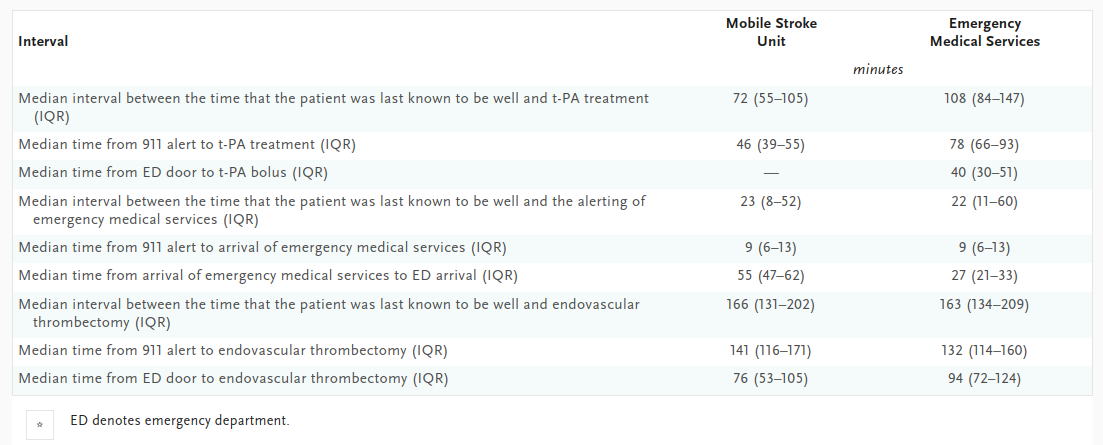
\includegraphics[width=0.75\linewidth]{images_background/best_msu_timings.png}
    \caption{BEST-MSU Timings}
    \label{fig:best_msu_timings}
\end{figure}

%%%%%%%%%%%%%%%%%%%%%%%%%%%%%%%%%%%%%%%%%% TELEMEDICINE %%%%%%%%%%%%%%%%%%%%%%%%%%%%%%%%%%%%%%%%%%
\subsection{MSU Telemedicine}

In a study of 174 patients in Houston, telemedicine neurologist assessment for a mobile stroke unit was reliable and fast \cite{wu_telemedicine_2017} . tPA decisions agreed 88\% of the time. NIHSS correlated well (0.88). Overall, there was disagreement in 20 of the 170 cases with decisions. In 13 out of 20 cases, the onboard vascular neurologist recommended tPA, whereas the telemedicine vascular neurologist did not. In 7 out of 20 cases, the telemedicine vascular neurologist recommended tPA whereas the onboard vascular neurologist did not. 

Bowry et al \cite{bowry_time_2018} compared time to decision in 50 patients in Houston. Time to tPA decision for the TM-VN was 21 minutes (interquartile range, 16.25–26) versus 18 minutes (interquartile range, 14–22) for the OB-VN (P=0.01). Initiation of tPA bolus was 24 minutes (interquartile range, 19.75–30) for the TM-VN versus 24 minutes (interquartile range, 19–27.75) for the OB-VN (P=0.5).

\subsection{Staffing of Mobile Stroke units}

\subsubsection{USA BEST-MSU Study}:

From [2]: Onboard staff typically includes emergency medical technicians or paramedics, a radiology technician, and nurse or nurse practitioner, in addition to a vascular neurologist.4 Some variants, such as that of the Cleveland Clinic, employ telemedicine consultation with the vascular neurologist. 


1. Emergency medical technicians (EMTs) or paramedics[2]
2. A radiology technician[2]
3. A nurse or nurse practitioner[2]
4. A vascular neurologist (either on-board or via telemedicine)[2][4]

Some key points about the staffing:

- The vascular neurologist could be physically present on the MSU or provide consultation via telemedicine, depending on the specific setup[2][4].

- The Cleveland Clinic variant of the MSU employed telemedicine consultation with the vascular neurologist rather than having them physically on board[2].

- Dr. Grotta's team demonstrated that assessment done through telemedicine was just as reliable as that of an on-board vascular neurologist[2].

- The MSU was equipped to function like a "primary stroke center emergency department on wheels" with this specialized team and resources to diagnose stroke and begin treatment before arriving at the hospital[6].

This staffing model allowed the MSU to provide clinical assessment, imaging diagnosis, and hyperacute treatment in the field, significantly reducing time to treatment for stroke patients compared to traditional emergency medical services[4][6].

Citations:
[1] https://pubmed.ncbi.nlm.nih.gov/26508753/
[2] https://practicalneurology.com/articles/2018-jan/mobile-stroke-units
[3] https://www.urmc.rochester.edu/stroke-center/mobile-stroke/about-msu/msu-q-a.aspx
[4] https://www.ncbi.nlm.nih.gov/pmc/articles/PMC9240459/
[5] https://pubmed.ncbi.nlm.nih.gov/34496173/
[6] https://www.uclahealth.org/news/article/new-study-shows-mobile-stroke-units-lead-to-better-patient-outcomes

\subsubsection{Berlin \cite{ebinger_effects_2015}}

* The MSU was staffed with a neurologist trained in emergency medicine, a
paramedic, and a radiology technician. A neuroradiologist was on call to evaluate images acquired on board the STEMO via a teleradiology connection.



%%%%%%%%%%%%%%%%%%%%%%%%%%%%%%%%%%%%%%%%%% THROMBECTOMY %%%%%%%%%%%%%%%%%%%%%%%%%%%%%%%%%%%%%%%%%%

\subsection{MSUs and thrombectomy}

The BEST-MSU substudy \cite{czap_abstract_2022} was a subset of the best MSU study, for tPA-eligible stroke patients with LVOs on CT and/or CTA. The study appeared to show MSUs have little effect on time to thrombectomy. A total of 295 patients were included, 169 in the MSU group and 126 in the EMS group. 92\% MSU vs 87\% EMS LVO patients received tPA, and 78\% vs 85\% went on to have EVT. MSU LVO patients had faster tPA bolus from symptom onset (65 min vs 96 min, p<0.001), however the two groups had similar onset to groin puncture (169 min vs 162 min, p=0.77). From the BEST study \cite{grotta_prospective_2021}, the median (and IQR) time from 911 alert to  thrombectomy was 141 (116–171) and 132 minutes (114–160) for MSU and EMS, and  time from ED door to thrombectomy was 76 (53–105) and 94 (72–124).

The Berlin study \cite{ebinger_association_2021} had MSU vs nomral care:

* Thrombectomy use: 13.8\% vs 14.2\%
* Dispatch to thrombectomy mins: 137 (117 to 166) vs 125 (110 to 154)


The Melbourne MSU study \cite{menezes_abstract_2023} found MSUs improved thrombectomy use and speed during, but not before, the COVID pandemic. A total of 402 patients (112 MSU) were included. Pre-pandemic, no reduction in dispatch to arterial access time was seen for MSU patients within an EVT centre catchment (median 11 min slower, p=0.38). However, a significant time saving was observed during the pandemic (median 29 min faster, p<0.001, p=0.0065). MSU care reduced hospital arrival to arterial access time by median 19 min pre-pandemic vs 40 min during the pandemic, p<0.001).

In Sydney the MSU did not improve time or rate of thrombectomy \cite{haliem_abstract_2023} but the MSU dispatch missed 40\% of those patients that would go on to receive thrombectomy. An odd finding there was also the ambo dispatch process was less likely to class severe strokes as stroke, compared to mild stroke. A total of n=618 patients were included with baseline NIHSS 16 (IQR 10-20). Of these, only 62\% (95\% CI 58-66) were initially dispatched as suspected stroke, with the most common non-stroke diagnoses being “Unconscious/Fainting” (19.2\%) and “Falls” (6.9\%). Those with a higher baseline severity (NIHSS $\ge$ 10) were less likely to be classified as stroke than those with lower severity (59\% vs 76\%, p<0.001), while no difference was found between metropolitan and rural patients (p=0.066). Overall, no significant time differences were found between stroke and non-stroke dispatches for ambulance dispatch to arterial access (median 208 vs 216 min, p=0.593) or hospital arrival to arterial access (median 42 vs 42 min, p=0.851). However, only 32 patients were treated on the MSU, which commenced operation November 2017 (2007-2021 was used for all data analysis). 


A review of available evidence suggests there is an evidence gap in MSUs and thrombectomy \cite{navi_mobile_2022}.




%%%%%%%%%%%%%%%%%%%%%%%%%%%%%%%%%%%%%%%%%% PICTURES %%%%%%%%%%%%%%%%%%%%%%%%%%%%%%%%%%%%%%%%%%

\begin{figure}
    \centering
    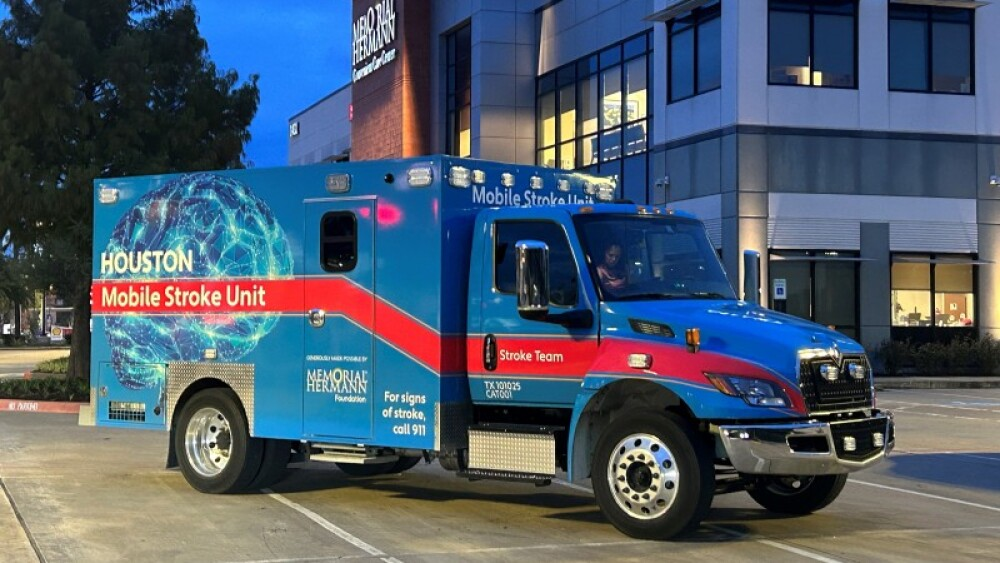
\includegraphics[width=0.5\linewidth]{images_background/houston_msu.jpeg}
    \caption{Houston Mobile Stroke Unit}
    \label{fig:houston_msu}
\end{figure}
